\documentclass{article}
\title{Informe Técnico Proyecto Ciencia de Datos}
\author{Clàudia Hernández Bayés}
\date{July 2024}

\usepackage{geometry}
  \geometry{
  a4paper,
  total={170mm, 257mm},
  left=20mm,
  top=20mm,
    }
    
\usepackage{booktabs}

\usepackage{Sweave}
\begin{document}
\Sconcordance{concordance:Informetecnico.tex:Informetecnico.Rnw:1 15 1 1 0 12 1 1 11 %
19 0 1 2 3 1 1 21 1 2 3 1 1 46 28 0 1 2 3 1 1 24 13 0 1 3 1 1 1 18 1 2 %
5 1}


\maketitle
\tableofcontents


\section*{Introducción}


\section*{Objetivo 1}
\subsection{Tabla Resumen}

% latex table generated in R 4.3.2 by xtable 1.8-4 package
% Wed Jul 24 12:53:39 2024
\begin{table}[ht]
\centering
\begin{tabular}{rr}
  \hline
essround & count \\ 
  \hline
2002 &  81 \\ 
  2004 &  71 \\ 
  2006 &  62 \\ 
  2008 &  89 \\ 
  2010 &  56 \\ 
  2012 &  65 \\ 
  2014 &  75 \\ 
  2016 & 119 \\ 
  2018 & 108 \\ 
  2020 & 286 \\ 
   \hline
\end{tabular}
\end{table}
En general, se observa una tendencia fluctuante en el número de casos de discriminación a lo largo de los años. A partir de 2014, hay un incremento significativo que alcanza su punto máximo en 2023 con 161 casos. Esto podría indicar un aumento en la concienciación y la denuncia de casos de discriminación, aunque también podría reflejar un incremento real en los incidentes de discriminación.En la siguiente gráfica podemos desglosar este recuento por tipo de discriminación. 

\subsection{Gráfico}
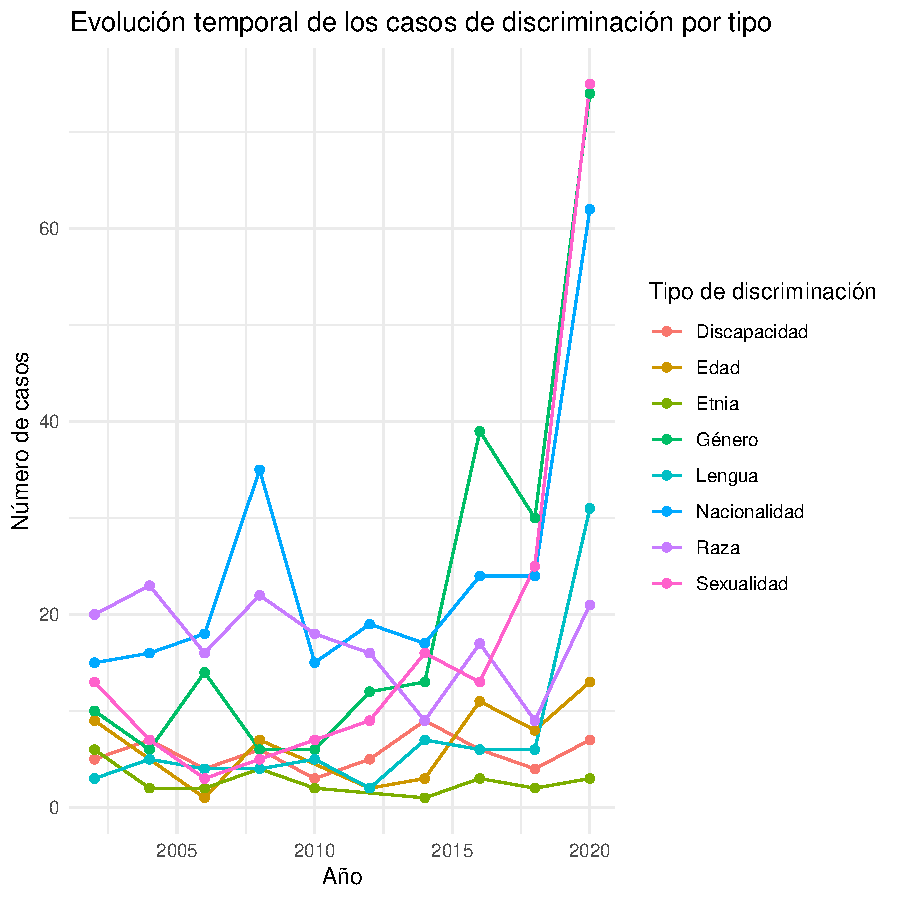
\includegraphics{Informetecnico-002}


\section*{Objetivo 2}
\subsection{Tabla Resumen}
% latex table generated in R 4.3.2 by xtable 1.8-4 package
% Wed Jul 24 12:53:39 2024
\begin{table}[ht]
\centering
\begin{tabular}{rrrr}
  \hline
region & casos & poblacion & tasa\_discriminacion \\ 
  \hline
Galicia &  47 & 2701743.00 & 1.74 \\ 
  Principado de Asturias &   9 & 1006193.00 & 0.89 \\ 
  Cantabria &  15 & 583904.00 & 2.57 \\ 
  País Vasco &  42 & 2188017.00 & 1.92 \\ 
  Comunidad Foral de Navarra &  11 & 661203.00 & 1.66 \\ 
  La Rioja &   7 & 319914.00 & 2.19 \\ 
  Aragón &  28 & 1320586.00 & 2.12 \\ 
  Comunidad de Madrid & 138 & 6714142.00 & 2.06 \\ 
  Castilla y León &  40 & 2394918.00 & 1.67 \\ 
  Castilla-La Mancha &  17 & 2046107.00 & 0.83 \\ 
  Extremadura &  11 & 1065424.00 & 1.03 \\ 
  Cataluña & 148 & 7739758.00 & 1.91 \\ 
  Comunitat Valenciana &  71 & 5057353.00 & 1.40 \\ 
  Illes Balears &  15 & 1172540.00 & 1.28 \\ 
  Andalucía &  81 & 8472403.00 & 0.96 \\ 
  Región de Murcia &  12 & 1511251.00 & 0.79 \\ 
  Ciudad de Ceuta &   1 & 84777.00 & 1.18 \\ 
  Ciudad de Melilla &   1 & 86384.00 & 1.16 \\ 
  Canarias &  15 & 2252465.00 & 0.67 \\ 
   \hline
\end{tabular}
\end{table}

\section*{Objetivo 3}
\subsection{Tabla Resumen}
% latex table generated in R 4.3.2 by xtable 1.8-4 package
% Wed Jul 24 12:53:39 2024
\begin{table}[ht]
\centering
\begin{tabular}{ccrr}
  \hline
pdjobev & discriminado & count & percentage \\ 
  \hline
Sí & No & 6050 & 95.61 \\ 
  Sí & Sí & 278 & 4.39 \\ 
  No & No & 2738 & 94.87 \\ 
  No & Sí & 148 & 5.13 \\ 
   \hline
\end{tabular}
\end{table}
\subsection{Gráfico}
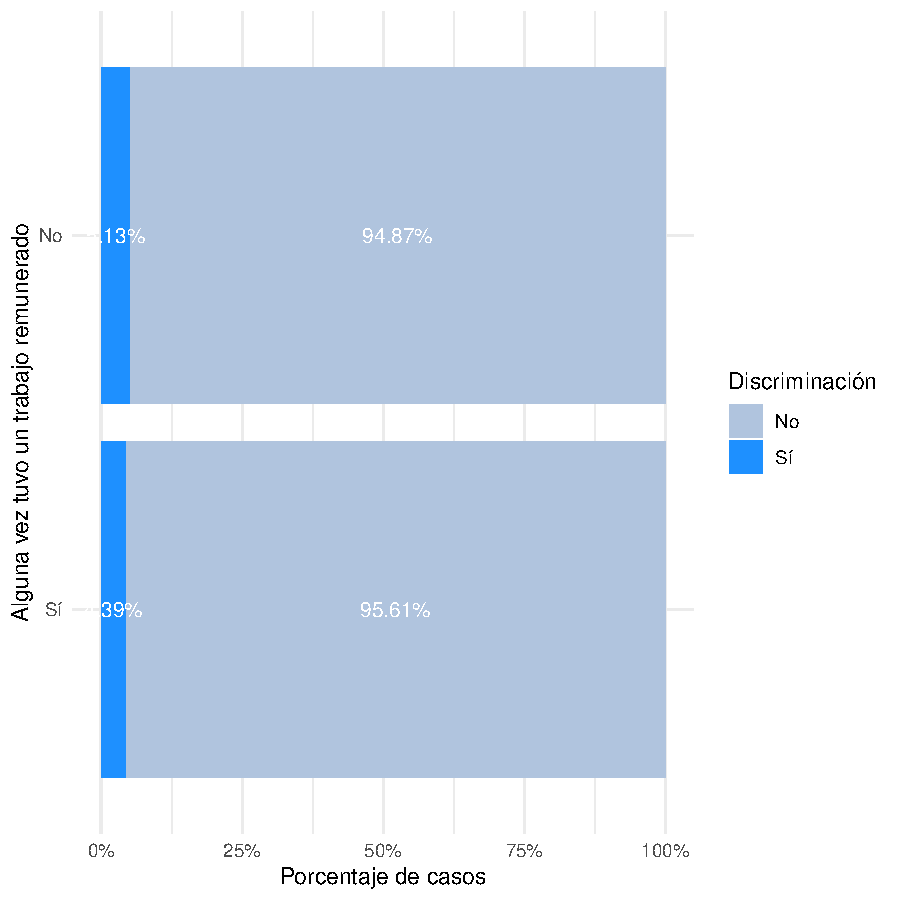
\includegraphics{Informetecnico-005}


\section*{Conclusiones}


\end{document}
